% +------------------------------------------------------------------------+
% | CGAL Reference Manual:  generators.tex
% +------------------------------------------------------------------------+
% | Geometric object generators.
% |
% | 09.06.1997   Lutz Kettner
% | 
\RCSdef{\generatorsRev}{$Revision$}
\RCSdefDate{\generatorsDate}{$Date$}
% +------------------------------------------------------------------------+

\beforecprogskip\medskipamount
\aftercprogskip\medskipamount
\ccParDims

\chapter{Geometric Object Generators}
\label{chapterGenerators}
\ccChapterRelease{\generatorsRev. \ \generatorsDate}\\
\ccChapterAuthor{Michael Hoffmann}\\
\ccChapterAuthor{Lutz Kettner}


A variety of generators for geometric objects is provided in \cgal.
They are useful as synthetic test data sets, e.g.~for testing
algorithms on degenerate object sets and for performance analysis.

The first section provides useful generic functions related to random
numbers like \ccc{CGAL_random_selection()}. The second section
documents generators for two-dimensional point sets, the third section
for three-dimensional point sets. The fourth section presents examples
using functions from Section~\ref{sectionGenericFunctions} to generate
composed objects, such as segments.  The fifth section describes
random convex sets.  Note that the \stl\ algorithm
\ccc{random_shuffle} is useful in this context to achieve random
permutations for otherwise regular generators (e.g.~points on a grid
or segment).

% +------------------------------------------------------------------------+
%\newpage
\section{Support Functions for Generators}
\ccThree{OutputIterator}{rand}{}


\subsection{{\it CGAL\_random\_selection()}}
\label{sectionRandomSelection}

\ccc{CGAL_random_selection} chooses $n$ items at random from a random
access iterator range which is useful to produce degenerate input data
sets with multiple entries of identical items.

\ccInclude{CGAL/random_selection.h}

\ccFunction{template <class RandomAccessIterator, class Size, 
                      class OutputIterator, class Random>
    OutputIterator CGAL_random_selection( RandomAccessIterator first,
        RandomAccessIterator last, 
        Size n, OutputIterator result, Random& rnd = default_random);}
{ chooses a random item from the range $[\ccc{first},\ccc{last})$ and
    writes it to \ccc{result}, each item from the range with equal
    probability, and repeats this $n$ times, thus writing $n$ items to
    \ccc{result}.
    A single random number is needed from \ccc{rnd} for each item.
    Returns the value of \ccc{result} after inserting the $n$ items.
    \ccPrecond \ccc{Random} is a random number generator type as provided 
    by the STL or by \ccc{CGAL_Random}.
}


% +------------------------------------------------------------------------+
\newpage
\section{2D Point Generators}
\label{sectionPointGenerators}

Two kind of point generators are provided: First, random point
generators and second deterministic point generators. Most random
point generators and a few deterministic point generators are provided
as input iterators.  The input iterators model an infinite sequence of
points. The function \ccc{CGAL_copy_n()} could be used to copy a
finite sequence, see Section~\ref{sectionCopyN}. The iterator adaptor
\ccc{CGAL_Counting_iterator} can be used to create finite iterator
ranges, see Section~\ref{sectionCountingIterator}.
Other generators are provided as functions writing to an output
iterator. Further functions add degeneracies or random perturbations.


% +------------------------------------------------------------------------+
\subsection{Point Generators as Input Iterators}

\ccDefinition

Input iterators are provided for random points uniformly distributed
over a two-dimensional domain (square or disc) or a one-dimensional
domain (boundary of a square, circle, or segment). Another input
iterator generates equally spaced points from a segment.

All iterators are parameterized with the point type \ccc{P} and all
with the exception of the class \ccc{CGAL_Points_on_segment_2} have a second
template argument \ccc{Creator} which defaults to the class
\ccc{CGAL_Creator_uniform_2<double,P>}\footnote{%
  For compilers not supporting these kind of default arguments, both
  template arguments must be provided when using these generators.}.
The \ccc{Creator} must be a function object accepting two \ccc{double}
values $x$ and $y$ and returning an initialized point \ccc{(x,y)} of type
\ccc{P}. Predefined implementations for these creators like the
default can be found in Section~\ref{sectionCreatorFunctionObjects}.
They simply assume an appropriate constructor for type \ccc{P}.

All generators know a range within which the coordinates of the
generated points will lie.

\ccInclude{CGAL/point_generators_2.h}

\ccTypes

The generators comply to the requirements of input iterators which
includes local type declarations including \ccc{value_type} which
denotes \ccc{P} here.

\ccCreation
\ccTwo{}{\hspace*{11cm}}
%% \ccTwo{}{\hspace*{10cm}}

\ccHtmlNoClassFile
\begin{ccClassTemplate}{CGAL_Random_points_in_disc_2<P,Creator>}
\ccCreationVariable{g}
\ccConstructor{CGAL_Random_points_in_disc_2( double r, CGAL_Random& rnd =
  default_random);}{%
  $g$ is an input iterator creating points of type \ccc{P} uniformly
  distributed in the open disc with radius $r$,
  i.e.~$|\ccc{*g}| < r$~. Two random numbers are needed from
  \ccc{rnd} for each point.
} 
\end{ccClassTemplate}

\ccHtmlNoClassFile
\begin{ccClassTemplate}{CGAL_Random_points_on_circle_2<P,Creator>}
\ccCreationVariable{g}
\ccConstructor{CGAL_Random_points_on_circle_2( double r, CGAL_Random& rnd =
  default_random);}{%
  $g$ is an input iterator creating points of type \ccc{P} uniformly
  distributed on the circle with radius $r$,
  i.e.~$|\ccc{*g}| == r$~. A single random number is needed from
  \ccc{rnd} for each point.
} 
\end{ccClassTemplate}

\ccHtmlNoClassFile
\begin{ccClassTemplate}{CGAL_Random_points_in_square_2<P,Creator>}
\ccCreationVariable{g}
\ccConstructor{CGAL_Random_points_in_square_2( double a, CGAL_Random& rnd =
  default_random);}{%
  $g$ is an input iterator creating points of type \ccc{P} uniformly
  distributed in the half-open square with side length $2 a$, centered
  at the origin, i.e.~$\forall p = \ccc{*g}:  -a \le p.x() < a$ and 
  $-a \le p.y() < a$~. 
  Two random numbers are needed from \ccc{rnd} for each point.
} 
\end{ccClassTemplate}

\ccHtmlNoClassFile
\begin{ccClassTemplate}{CGAL_Random_points_on_square_2<P,Creator>}
\ccCreationVariable{g}
\ccConstructor{CGAL_Random_points_on_square_2( double a, CGAL_Random& rnd =
  default_random);}{%
  $g$ is an input iterator creating points of type \ccc{P} uniformly
  distributed on the boundary of the square with side length $2 a$,
  centered at the origin, i.e.~$\forall p = \ccc{*g}:$ one
  coordinate is either $a$ or $-a$ and for the 
  other coordinate $c$ holds $-a \le c < a$~.
  A single random number is needed from \ccc{rnd} for each point.
} 
\end{ccClassTemplate}

\ccHtmlNoClassFile
\begin{ccClassTemplate}{CGAL_Random_points_on_segment_2<P,Creator>}
\ccCreationVariable{g}
\ccConstructor{CGAL_Random_points_on_segment_2( const P& p, const P& q,
  CGAL_Random& rnd = default_random);}{%
  $g$ is an input iterator creating points of type \ccc{P} uniformly
  distributed on the segment from $p$ to $q$ (excluding $q$),
  i.e.~$\ccc{*g} == (1-\lambda)\, p + \lambda q$ where $0 \le \lambda < 1$~.
  A single random number is needed from \ccc{rnd} for each point.
  \ccPrecond The expressions \ccc{CGAL_to_double(p.x())} and
    \ccc{CGAL_to_double(p.y())} must  result in the respective
    \ccc{double} representation of the coordinates and similar for $q$.}

\end{ccClassTemplate}

\ccHtmlNoClassFile
\begin{ccClassTemplate}{CGAL_Points_on_segment_2<P>}
\ccCreationVariable{g}
\ccConstructor{CGAL_Points_on_segment_2( const P& p, const P& q, 
                                         size_t n, size_t i = 0);}{%
  $g$ is an input iterator creating points of type \ccc{P} equally 
  spaced on the segment from $p$ to $q$. $n$ points are placed on the
  segment including $p$ and $q$. The iterator denoted the point $i$
  where $p$ has the index 0 and $q$ the index $n$.
  \ccPrecond The expressions \ccc{CGAL_to_double(p.x())} and
    \ccc{CGAL_to_double(p.y())} must  result in the respective
    \ccc{double} representation of the coordinates and similar for $q$.}


\ccOperations
\ccThree{double}{g.source();}{}

\ccMethod{double range();}{returns the range in which the point
  coordinates lie, i.e.~$\forall x: |x| \leq $\ccc{range()} and
  $\forall y: |y| \leq $\ccc{range()}.}

The generators \ccc{CGAL_Random_points_on_segment_2} and
\ccc{CGAL_Points_on_segment_2} have to additional methods.

\ccMethod{const P& source();}{returns the source point of the segment.}
\ccGlue
\ccMethod{const P& target();}{returns the target point of the segment.}

\end{ccClassTemplate}


\ccSeeAlso

\ccc{stl::random_shuffle}, \ccc{CGAL_random_selection}, 
\ccc{CGAL_copy_n}, \ccc{CGAL_Counting_iterator},
\ccTexHtml{\\}{}
\ccc{CGAL_Join_input_iterator_1}.


% +------------------------------------------------------------------------+
\subsection{Point Generators as Functions}

\ccHeading{Grid Points}
\ccThree{OutputIterator}{rand}{}

Grid points are generated by functions writing to an output iterator.

\def\ccLongParamLayout{\ccTrue}
\ccFunction{template <class OutputIterator, Creator creator>
    OutputIterator
    CGAL_points_on_square_grid_2( double a, size_t n, OutputIterator o,
                                  Creator creator = 
                                  CGAL_Creator_uniform_2<double,P>);}
{ creates the $n$ first points on the regular $\lceil\sqrt{n}\,\rceil
    \times \lceil  \sqrt{n}\,\rceil$ grid within the square
    $[-a,a]\times [-a,a]$. Returns the value of $o$ after inserting
    the $n$ points. 
    \ccPrecond \ccc{Creator} must be a function object accepting two
    \ccc{double} values $x$ and $y$ and returning an initialized point
    \ccc{(x,y)} of type \ccc{P}. Predefined implementations for these
    creators like the default can be found in
    Section~\ref{sectionCreatorFunctionObjects}. The
    \ccc{OutputIterator} must accept values of type \ccc{P}. If the
    \ccc{OutputIterator} has a \ccc{value_type} the default
    initializer of the \ccc{creator} can be used. \ccc{P} is set to
    the \ccc{value_type} in this case.}
\def\ccLongParamLayout{\ccFalse}


\ccFunction{template <class P, class OutputIterator>
    OutputIterator CGAL_points_on_segment_2( const P& p, const P& q, size_t n,
    OutputIterator o);}
{ creates $n$ points equally spaced on the segment from $p$ to $q$,
    i.e.~$\forall i: 0 \le i < n: o[i] := \frac{n-i-1}{n-1}\, p +
    \frac{i}{n-1}\, q$. Returns the value of $o$ after inserting
    the $n$ points.}

\ccHeading{Random Perturbations}

Degenerate input sets like grid points can be randomly perturbed by a
small amount to produce {\em quasi}-degenerate test sets. This
challenges numerical stability of algorithms using inexact arithmetic and
exact predicates to compute the sign of expressions slightly off from zero.

\ccFunction{template <class ForwardIterator>
    void CGAL_perturb_points_2( ForwardIterator first, ForwardIterator last, 
        double xeps, double yeps = xeps, CGAL_Random& rnd = default_random,
        Creator creator = CGAL_Creator_uniform_2<double,P>);}
{ perturbs the points in the range $[\ccc{first},\ccc{last})$ by
  replacing each point with a random point from the rectangle
  \ccc{xeps} $\times$ \ccc{yeps} centered at the original point.
  Two random numbers are needed from \ccc{rnd} for each point.
  \ccPrecond   \ccc{Creator} must be a function object accepting two
    \ccc{double} values $x$ and $y$ and returning an initialized point
    \ccc{(x,y)} of type \ccc{P}. Predefined implementations for these
    creators like the default can be found in
    Section~\ref{sectionCreatorFunctionObjects}. The \ccc{value_type} of the
    \ccc{ForwardIterator} must be assignable to \ccc{P}.
    \ccc{P} is equal to the \ccc{value_type} of the
    \ccc{ForwardIterator} when using the default initializer.
    The expressions \ccc{CGAL_to_double((*first).x())} and
    \ccc{CGAL_to_double((*first).y())} must result in the respective
    coordinate values.
}

\ccHeading{Adding Degeneracies}

For a given point set certain kinds of degeneracies can be produced
adding new points. The \ccc{CGAL_random_selection()} function is
useful to generate multiple entries of identical points, see
Section~\ref{sectionRandomSelection}. The
\ccc{CGAL_random_collinear_points_2()} function adds collinearities to
a point set.


\def\ccLongParamLayout{\ccTrue}
\ccFunction{template <class RandomAccessIterator, class OutputIterator>
    OutputIterator CGAL_random_collinear_points_2( RandomAccessIterator first,
        RandomAccessIterator last, 
        size_t n, OutputIterator first2, CGAL_Random& rnd = default_random,
        Creator creator = CGAL_Creator_uniform_2<double,P>);}
{ randomly chooses two points from the range $[\ccc{first},\ccc{last})$,
    creates a random third point on the segment connecting this two
    points, writes it to \ccc{first2}, and repeats this $n$ times, thus
    writing $n$ points to \ccc{first2} that are collinear with points
    in the range $[\ccc{first},\ccc{last})$.
    Three random numbers are needed from \ccc{rnd} for each point.
    Returns the value of \ccc{first2} after inserting the $n$ points.
  \ccPrecond  \ccc{Creator} must be a function object accepting two
    \ccc{double} values $x$ and $y$ and returning an initialized point
    \ccc{(x,y)} of type \ccc{P}. Predefined implementations for these
    creators like the default can be found in
    Section~\ref{sectionCreatorFunctionObjects}. The \ccc{value_type} of the
    \ccc{RandomAccessIterator} must be assignable to \ccc{P}.
    \ccc{P} is equal to the \ccc{value_type} of the
    \ccc{RandomAccessIterator} when using the default initializer.
    The expressions \ccc{CGAL_to_double((*first).x())} and
    \ccc{CGAL_to_double((*first).y())} must result in the respective
    coordinate values.
}
\def\ccLongParamLayout{\ccFalse}


\ccSeeAlso

\ccc{stl::random_shuffle}, \ccc{CGAL_random_selection}.

\ccExample

We want to generate a test set of 1000 points, where 60\% are chosen
randomly in a small disc, 20\% are from a larger grid, 10\% duplicates
are added, and 10\% collinearities added. A random shuffle removes the
construction order from the test set. See \ccTexHtml{%
Figure~\ref{figurePointGenerator}}{Figure <A HREF="#PointGenerators">
  <IMG SRC="cc_ref_up_arrow.gif" ALT="reference arrow" WIDTH="10"
  HEIGHT="10"></A>} for the example output.

\cprogfile{generators_prog1.C}

\begin{ccTexOnly}
  \begin{figure}
    \noindent
    \hspace*{0.025\textwidth}%
    \begin{minipage}{0.45\textwidth}%
      \includegraphics[width=\textwidth]{generators_prog1.ps}
      \caption{Output of example program for point generators.}
      \label{figurePointGenerator}
    \end{minipage}%
    \hspace*{0.05\textwidth}%
    \begin{minipage}{0.45\textwidth}%
      \includegraphics[width=\textwidth]{generators_prog2.ps}
      \caption{Output of example program for point generators working
        on integer points.}
      \label{figureIntegerPointGenerator}
    \end{minipage}%
  \end{figure}
\end{ccTexOnly}

\begin{ccHtmlOnly}
  <A NAME="PointGenerators">
  <TABLE><TR><TD ALIGN=LEFT VALIGN=TOP WIDTH=60%>
    <A HREF="./generators_prog1.gif">Figure:</A>
    Output of example program for point generators.
  </TD><TD ALIGN=LEFT VALIGN=TOP WIDTH=5% NOWRAP>
  </TD><TD ALIGN=LEFT VALIGN=TOP WIDTH=35% NOWRAP>
    <A HREF="./generators_prog1.gif">
        <img src="./generators_prog1_small.gif" 
             alt="Point Generator Example Output"></A>
  </TD></TR></TABLE>
\end{ccHtmlOnly}

\newpage

The second example demonstrates the point generators with integer
points. Arithmetic with \ccc{double}'s is sufficient to produce
regular integer grids. See \ccTexHtml{%
Figure~\ref{figureIntegerPointGenerator}}{Figure 
  <A HREF="#IntegerPointGenerators">
  <IMG SRC="cc_ref_up_arrow.gif" ALT="reference arrow" WIDTH="10"
  HEIGHT="10"></A>}
for the example output.

\cprogfile{generators_prog2.C}

\begin{ccHtmlOnly}
  <A NAME="IntegerPointGenerators">
  <TABLE><TR><TD ALIGN=LEFT VALIGN=TOP WIDTH=60%>
    <A HREF="./generators_prog2.gif">Figure:</A>
        Output of example program for point generators working
        on integer points.
  </TD><TD ALIGN=LEFT VALIGN=TOP WIDTH=5% NOWRAP>
  </TD><TD ALIGN=LEFT VALIGN=TOP WIDTH=35% NOWRAP>
    <A HREF="./generators_prog2.gif">
        <img src="./generators_prog2_small.gif" 
             alt="Integer Point Generator Example Output"></A>
  </TD></TR></TABLE>
\end{ccHtmlOnly}


% +------------------------------------------------------------------------+
\newpage
\section{3D Point Generators}

One kind of point generators is currently provided: Random point
generators implemented as input iterators.  The input iterators model
an infinite sequence of points. The function \ccc{CGAL_copy_n()} could
be used to copy a finite sequence, see Section~\ref{sectionCopyN}. The
iterator adaptor \ccc{CGAL_Counting_iterator} can be used to create
finite iterator ranges, see Section~\ref{sectionCountingIterator}.


% +------------------------------------------------------------------------+
\subsection{Point Generators as Input Iterators}

\ccDefinition

Input iterators are provided for random points uniformly distributed
in a three-dimensional volume (sphere or cube) or a two-dimensional
surface (boundary of a sphere).

All iterators are parameterized with the point type \ccc{P} and a second
template argument \ccc{Creator} which defaults to
\ccc{CGAL_Creator_uniform_3<double,P>}\footnote{%
  For compilers not supporting these kind of default arguments, both
  template arguments must be provided when using these generators.}.
The \ccc{Creator} must be a function object accepting three
\ccc{double} values $x$, $y$ and $z$ and returning an initialized
point \ccc{(x,y,z)} of type \ccc{P}. Predefined implementations for
these creators like the default can be found in
Section~\ref{sectionCreatorFunctionObjects}.  They simply assume an
appropriate constructor for type \ccc{P}.

All generators know a range within which the coordinates of the
generated points will lie.

\ccInclude{CGAL/point_generators_3.h}

\ccTypes

The generators comply to the requirements of input iterators which
includes local type declarations including \ccc{value_type} which
denotes \ccc{P} here.

\ccCreation
\ccTwo{}{\hspace*{11cm}}

\ccHtmlNoClassFile
\begin{ccClassTemplate}{CGAL_Random_points_in_sphere_3<P,Creator>}
\ccCreationVariable{g}
\ccConstructor{CGAL_Random_points_in_sphere_3( double r, CGAL_Random& rnd =
  default_random);}{%
  $g$ is an input iterator creating points of type \ccc{P} uniformly
  distributed in the open sphere with radius $r$,
  i.e.~$|\ccc{*g}| < r$~. 
} 
\end{ccClassTemplate}

\ccHtmlNoClassFile
\begin{ccClassTemplate}{CGAL_Random_points_on_sphere_3<P,Creator>}
\ccCreationVariable{g}
\ccConstructor{CGAL_Random_points_on_sphere_3( double r, CGAL_Random& rnd =
  default_random);}{%
  $g$ is an input iterator creating points of type \ccc{P} uniformly
  distributed on the boundary of a sphere with radius $r$,
  i.e.~$|\ccc{*g}| == r$~. Two random numbers are needed from
  \ccc{rnd} for each point.
} 
\end{ccClassTemplate}

\ccHtmlNoClassFile
\begin{ccClassTemplate}{CGAL_Random_points_in_cube_3<P,Creator>}
\ccCreationVariable{g}
\ccConstructor{CGAL_Random_points_in_cube_3( double a, CGAL_Random& rnd =
  default_random);}{%
  $g$ is an input iterator creating points of type \ccc{P} uniformly
  distributed in the half-open cube with side length $2 a$, centered
  at the origin, i.e.~$\forall p = \ccc{*g}:  -a \le p.x(),p.y(),p.z() < a$~. 
  Three random numbers are needed from \ccc{rnd} for each point.
} 
\end{ccClassTemplate}


\ccSeeAlso

\ccc{stl::random_shuffle}, \ccc{CGAL_random_selection}, 
\ccc{CGAL_copy_n}, \ccc{CGAL_Counting_iterator}, 
\ccTexHtml{\\}{}
\ccc{CGAL_Join_input_iterator_1}.


% +------------------------------------------------------------------------+
\newpage
\section{Examples Generating Segments}

The following two examples illustrate the use of the generic functions
from Section~\ref{sectionGenericFunctions} like
\ccc{CGAL_Join_input_iterator} to generate composed objects from other
generators -- here two-dimensional segments from two point generators.

We want to generate a test set of 200 segments, where one endpoint is
chosen randomly from a horizontal segment of length 200, and the other
endpoint is chosen randomly from a circle of radius 250. See
\ccTexHtml{Figure~\ref{figureSegmentGenerator}}{Figure <A
  HREF="#SegmentGenerator"> <IMG SRC="cc_ref_up_arrow.gif"
  ALT="reference arrow" WIDTH="10" HEIGHT="10"></A>} for the example
output.

\begin{ccTexOnly}
  \begin{figure}
    \noindent
    \hspace*{0.025\textwidth}%
    \begin{minipage}[t]{0.45\textwidth}%
      \includegraphics[width=\textwidth]{Segment_generator_prog1.ps}
      \caption{Output of the first example program for the generic generator.}
      \label{figureSegmentGenerator}
    \end{minipage}%
    \hspace*{0.05\textwidth}%
    \begin{minipage}[t]{0.45\textwidth}%
      \includegraphics[width=\textwidth]{Segment_generator_prog2.ps}
      \caption{Output of the second example program for the generic
        generator without using intermediate storage.}
      \label{figureSegmentGeneratorFan}
    \end{minipage}%
  \end{figure}
\end{ccTexOnly}

\cprogfile{Segment_generator_prog1.C}

\begin{ccHtmlOnly}
  <A NAME="SegmentGenerator">
  <TABLE><TR><TD ALIGN=LEFT VALIGN=TOP WIDTH=60%>
    <A HREF="./Segment_generator_prog1.gif">Figure:</A>
    Output of example program for the generic segment generator.
  </TD><TD ALIGN=LEFT VALIGN=TOP WIDTH=5% NOWRAP>
  </TD><TD ALIGN=LEFT VALIGN=TOP WIDTH=35% NOWRAP>
    <A HREF="./Segment_generator_prog1.gif">
        <img src="./Segment_generator_prog1_small.gif" 
             alt="Segment Generator Example Output"></A>
  </TD></TR></TABLE>
\end{ccHtmlOnly}

The second example generates a regular structure of 100 segments, see 
\ccTexHtml{Figure~\ref{figureSegmentGeneratorFan}}{Figure <A
  HREF="#SegmentGeneratorFan"> <IMG SRC="cc_ref_up_arrow.gif"
  ALT="reference arrow" WIDTH="10" HEIGHT="10"></A>} for the example
output. It uses the \ccc{CGAL_Points_on_segment_2} iterator,
\ccc{CGAL_Join_input_iterator_2} and \ccc{CGAL_Counting_iterator} to
avoid any intermediate storage of the generated objects until they are
used, in this example copied to a window stream.

\cprogfile{Segment_generator_prog2.C}

\begin{ccHtmlOnly}
  <A NAME="SegmentGeneratorFan">
  <TABLE><TR><TD ALIGN=LEFT VALIGN=TOP WIDTH=60%>
    <A HREF="./Segment_generator_prog2.gif">Figure:</A>
    Output of example program for the generic segment generator using
    pre-computed point locations.
  </TD><TD ALIGN=LEFT VALIGN=TOP WIDTH=5% NOWRAP>
  </TD><TD ALIGN=LEFT VALIGN=TOP WIDTH=35% NOWRAP>
    <A HREF="./Segment_generator_prog2.gif">
        <img src="./Segment_generator_prog2_small.gif" 
             alt="Segment Generator Example Output 2"></A>
  </TD></TR></TABLE>
\end{ccHtmlOnly}


% +--------------------------------------------------------+
% restore default column and paragraph layout
\ccParDims
\cgalColumnLayout
\beforecprogskip\parskip
\aftercprogskip0pt

%% ==============================================================
%% Specification: Random Convex Sets
%% --------------------------------------------------------------
%% file  : rcs_spec.awi
%% author: Michael Hoffmann
%% maintainer: Susan Hert 
%% $Id$
%% ==============================================================

\RCSdef{\RandomConvexSetRev}{$Revision$}
\RCSdefDate{\RandomConvexSetDate}{$Date$}

\newpage

\ccParDims

\section{Building Random Convex Sets}
\label{section_BuildingRandomConvexSets}
\lcTex{\ccIndexMainItem[c]{random convex set}}

This section describes a function to compute a random convex planar
point set of given size where the points are drawn from a specific
domain.

\ccInclude{CGAL/random_convex_set_2.h}

\def\ccLongParamLayout{\ccTrue} 

\ccGlobalFunction{template < class OutputIterator, class Point_generator,
  class Traits > OutputIterator random_convex_set_2( int n,
  OutputIterator o, const Point_generator& pg, Traits t =
  Default_traits);}

computes a random convex \ccc{n}-gon by writing its vertices (oriented
counterclockwise) to \ccc{o}. The resulting polygon is scaled such
that it fits into the bounding box as specified by \ccc{pg}. Therefore
we cannot easily describe the resulting distribution.

\ccHeading{Precondition}
\begin{enumerate}
\item \ccc{Point_generator} satisfies the requirements stated in
  section \ref{point_generator_req},
\item If \ccc{Traits} is specified, it has to satisfy the
  requirements stated in section \ref{req_random_convex_sets_traits}
  and \ccc{Traits::Point_2} must be the same as
  \ccc{Point_generator::value_type},
\item if \ccc{Traits} is not specified,
  \ccc{Point_generator::value_type} must be \ccc{Point_2<
    R >} for some representation class \ccc{R},
\item \ccc{OutputIterator} accepts
  \ccc{Point_generator::value_type} as value type {\it and}
\item $n \ge 3$.
\end{enumerate}

\ccSeeAlso \ccc{Random_points_in_square_2} and
\ccc{Random_points_in_disc_2}.

\ccImplementation The implementation uses the centroid method
described in \cite{s-zkm-96} and has a worst case running time of $O(r
\cdot n + n \cdot \log n)$, where $r$ is the time needed by \ccc{pg}
to generate a random point.

\ccExample

The following program displays a random convex 500-gon where the
points are drawn uniformly from the unit square centered at the
origin.

\ccIncludeVerbatim{rcs_prog.C}

\ccTagDefaults

\begin{ccClass}{Point_generator}
    \ccCreationVariable{pg} \ccTagFullDeclarations
    
    \ccSubsection{Requirements for Point Generator
      Classes}\label{point_generator_req}
    \lcTex{\ccIndexMainItem{generator classes, requirements}}
    
    \ccDefinition A class \ccClassName\ satisfying input iterator
    requirements has to provide the following additional types and
    operations in order to qualify as a point generator class. The
    point generators described in section \ref{sectionPointGenerators}
    fulfill these requirements.

    \ccTypes\lcTex{\ccIndexClassTypes}
    
    \ccNestedType{value_type}{point class.}  
    
    \ccNestedType{FT}{class used for doing computations on point
      coordinates (has to fulfill field type requirements).}

    \ccOperations
    \lcTex{\begin{ccIndexMemberFunctions}}
    
    \ccMemberFunction{FT range() const;}{return an absolute bound for
      the coordinates of all generated points.}
    \lcTex{\end{ccIndexMemberFunctions}}
    
\end{ccClass}

\begin{ccAdvanced}
  \lcTex{\ccAutoIndexingOff}
  \ccHtmlNoIndex\ccHtmlNoClassLinks\begin{ccClass}{Traits}
    \ccCreationVariable{t}
    \ccTagFullDeclarations
    
    \subsection{Requirements for Random Convex Sets Traits
      Classes}\label{req_random_convex_sets_traits}%
      \lcTex{\ccIndexSubitem[c]{random convex set}{traits requirements}}
    
    \ccDefinition A class \ccClassName\ has to provide the following
    types and operations in order to qualify as a traits class for
    \ccc{random_convex_set_2}.
    
    \ccTypes 
    
    \ccNestedType{Point_2}{point class.}
    \ccNestedType{FT}{class used for doing computations on point and
      vector coordinates (has to fulfill field type requirements).}
    
    \ccNestedType{Sum}{AdaptableBinaryFunction class:
      \ccc{Point_2} $\times$ \ccc{Point_2} $\rightarrow$
      \ccc{Point_2}. It returns the point that results from adding
      the vectors corresponding to both arguments.}
    
    \ccNestedType{Scale}{AdaptableBinaryFunction class:
      \ccc{Point_2} $\times$ \ccc{FT} $\rightarrow$
      \ccc{Point_2}. \ccc{Scale(p,k)} returns the point that
      results from scaling the vector corresponding to \ccc{p} by a
      factor of \ccc{k}.}
    
    \ccNestedType{Max_coordinate}{AdaptableUnaryFunction class:
      \ccc{Point_2} $\rightarrow$ \ccc{FT}. \ccc{Max_coordinate(p)}
      returns the coordinate of \ccc{p} with largest absolute value.}

    \ccNestedType{Angle_less}{AdaptableBinaryFunction class:
      \ccc{Point_2} $\times$ \ccc{Point_2} $\rightarrow$
      \ccc{bool}. It returns \ccc{true}, iff the angle of the
      direction corresponding to the first argument with respect to
      the positive $x$-axis is less than the angle of the direction
      corresponding to the second argument.}

    \ccOperations
    
    \ccMemberFunction{Point_2 origin() const;}{return origin (neutral
      element for the \ccc{Sum} operation).}
      
  \end{ccClass}
  \lcTex{\ccAutoIndexingOn}
\end{ccAdvanced}

%% EOF %%



% +--------------------------------------------------------+
% restore default column and paragraph layout
\ccParDims
\beforecprogskip\parskip
\aftercprogskip0pt


% EOF
